\chapter{Backend and Runtime}
\label{chapter:backend-and-runtime}

This chapter discusses the last component of the SableWasm compilation pipeline:
the code generation backend and runtime support for generated shared libraries.
Currently, SableWasm has only one backend based on the LLVM compiler
infrastructure. However, in the future, one can easily extend the system by
adding more backends that lower SableWasm MIR into other target languages.
Another problem that appears when designing a backend is how SableWasm MIR
entities map to native constructs. In SableWasm, we take an instance-based
approach. The SableWasm runtime library will manage all entities in an instance
object. The system will pass it to the generated native functions as the first
argument, similar to `this' pointer in many C++ implementations. In the rest of
this chapter, we will first go through the design of the instance object,
followed by the implementation of WebAssembly entities. Finally, we will
discuss the code generation strategies used when lowering SableWasm MIR to LLVM
intermediate representation and the interaction between generated shared
libraries and the hosting language.

\section{Instance Layout}
\label{section:runtime-instance-layout}

\begin{figure}
    \begin{minipage}{.35\textwidth}
        \centering
        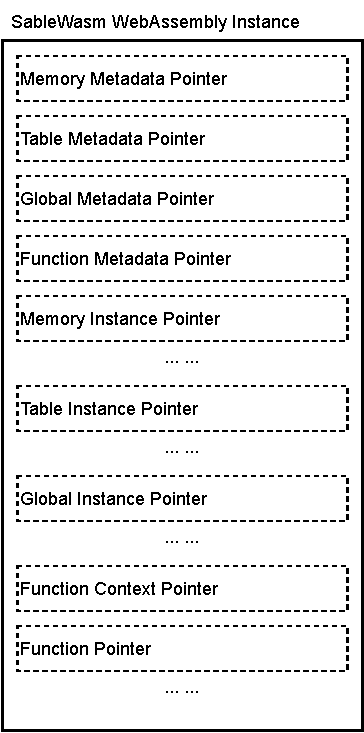
\includegraphics[
            width=\textwidth
        ]{Images/5.Backend and Runtime/instance}
    \end{minipage}\hfill
    \begin{minipage}{.6\textwidth}
        \begin{lstlisting}[
            language=C, 
            basicstyle=\linespread{1}\ttfamily\footnotesize]
struct instance {
    memory_metadata_t   *memory_metadata;
    table_metadata_t    *table_metadata;
    global_metadata_t   *global_metadata;
    function_metadata_t *function_metadata;
    memory_t            *memories[NUM_MEMORY];
    table_t             *tables[NUM_TABLE];
    global_t            *globals[NUM_GLOBAL];
    struct {
        struct instance *context;
        function_t      *function_ptr;
    } *functions[NUM_FUNCTIONS];
};        
    \end{lstlisting}
    \end{minipage}
    \caption{SableWasm WebAssembly instance}
    \label{fig:backend-instance}
\end{figure}

This section discusses the WebAssembly instance implementation in SableWasm.
A WebAssembly instance hosts all the runtime structures that the generated
shared libraries require, such as linear memories and indirect tables.
Figure~\ref{fig:backend-instance} illustrates the design of the WebAssembly
instance. SableWasm's WebAssembly instance object consists of two parts,
metadata entries and entity pointers. One may also notice that the instance
object's size may vary from one module to another depending on how many entities
are declared. This behaviour is intentional by design. The SableWasm runtime
system needs to compute the address of the pointers based on the metadata
information on the fly. By packing all pointers in a consecutive memory region,
we reduce one layer of indirection for the runtime system, and in theory, may
improve runtime performance. On the other hand, the generated shared library
has all the entities address inlined as the backend can compute them during code
generation, which does not incur any performance loss. For most of the entities,
they are pretty straightforward, and we will skip the discussion here. In the
rest of the section, we focus on three aspects: the metadata entries,
the function entity representations, and the instance initialization protocol
in SableWasm.

\paragraph{Metadata}
One could think of the metadata as the signatures for entities, and indeed, the
SableWasm runtime system prepares the instance object based on the metadata.
Further, shared libraries generated by SableWasm only publicly expose the
metadata and initialization function to conceal module details. Metadata encodes
the type for the entity. For linear memories and indirect tables, this is
relatively trivial as their types only consist of an integer pair. In the case
of global variables, things are a little bit complicated. A quick reminder,
WebAssembly global variable types keep track of their value type and mutability.
The first problem here is how to encode WebAssembly value types. One solution is
to use WebAssembly value type binary format. However, this encoding strategy is
hard to maintain as a human cannot directly read them. Here we use the JVM
approach for value type encoding
\footnote{\url{https://docs.oracle.com/javase/7/docs/technotes/
        guides/jni/spec/types.html}}. In short, in SableWasm, we encode
32-bit integers as `I', 64-bit integers as 'J', single-precision floating-point
numbers as 'F', double-precision floating-point numbers as 'D', and finally,
128-bit vectors as 'V'. The second problem is how to encode mutability. In
SableWasm, we use capital letters for constant global variable types and lower
letters for mutable ones. Finally, for function types, we follow a similar
design as we used for global variables. SableWasm encodes a function type into a
null-terminated string. Let's take \texttt{[i32, f32] -> [v128]} as an example.
SableWasm encodes the type into `\texttt{IF:V}'. The colon acts as a separator
between parameter types and result types. Note that `\texttt{:}' itself is also
a valid SableWasm function signature string, and represents \texttt{[] -> []},
a void function with no arguments. Finally, metadata also encodes module names
and entity names for import entities and names for export entities, which play
a critical role later in the module initialization phase.

\paragraph{Function entity representation}
The WebAssembly specification classifies the functions into two groups,
WebAssembly functions and host functions. WebAssembly functions are any
functions defined within a WebAssembly module. On the other hand, host
functions are directly provided by the host system, and from the WebAssembly
module's perspective, the host functions are black boxes without any knowledge
of their internals. Making things more complex, in MVP WebAssembly, there are no
explicit requirements on how the WebAssembly functions should behave if they
are invoked from other modules. Here we use a similar generalization like the
one adopted by Javascript \footnote{WebAssembly Javascript Interface:
    \url{https://www.w3.org/TR/wasm-js-api-1/}}. In short, in SableWasm, if a
module exports a function, it exports the function in a closure that captures
its enclosing instance. Suppose a second module invokes the exported closure
as an import function. In this case, the function still only has access to its
original module's entities and only communicates to the second module via
return values. Hence, in SableWasm, we implement our function as a pair of
pointers. The first one refers to its enclosing instance, and the second one
relates to the generated function code. In this chapter's introduction, we
mentioned that we pass the instance object as the first argument to the
generated functions upon function calls. But, what should we give to the host
function invocations? SableWasm defines that for all the host functions, the
instance object pointer will always point to the caller's enclosing instance
so that the host functions can access the internals of the caller's module.

\paragraph{Initialization protocol}
In the last part of the section, we will cover the initialization protocol we
used in SableWasm. The initialization protocol consists of three basic steps:
validation, instance preparation, and initialization.
In the validation phase, we load the shared library with the operating system's
help, such as \texttt{dlopen} on Linux, and check if it contains all the
required symbols. Currently, a SableWasm shared library needs to export five
symbols in total. Table~\ref{tbl:sablewasm-runtime-export-syms} illustrates the
symbols expected from the generated shared libraries. The instance initializer
function takes a \emph{prepared} instance object as the argument. The next step
in SableWasm is to construct this \emph{prepared} instance object. The idea of
a \emph{prepared} instance object is that we want to separate the memory
allocation from the value initialization. In SableWasm, the runtime system
handles the memory allocation, while on the other hand, the initializer function
takes care of the value initialization. In the second phase, the SableWasm
runtime allocates all the entities and attaches them to the module instance.
Note that SableWasm also resolves all the import names at this stage, and it
will only proceed to the next step if all the expecting import entities are set.
The import name binding utilizes the module names and entity names provided by
the metadata. Finally, the last step is the initialization. SableWasm will
invoke the initializer function supplied by the shared library. The initializer
function takes care of all kinds of value initialization, such as setting values
for global variables and copying data segments into linear memories. If the
runtime system adequately prepares the instance context, the initializer
function should never fail.

\begin{table}[h]
    \centering
    \begin{tabular}{|l|l|}
        \hline
        \textbf{Symbol Name}          & \textbf{Description}          \\ \hline
        \_\_sable\_global\_metadata   & Metadata for global values    \\ \hline
        \_\_sable\_memory\_metadata   & Metadata for linear memories  \\ \hline
        \_\_sable\_table\_metadata    & Metadata for indirect tables  \\ \hline
        \_\_sable\_function\_metadata & Metadata for functions        \\ \hline
        \_\_sable\_initialize         & Instance initializer function \\ \hline
    \end{tabular}
    \caption{SableWasm shared libraries exported symbols}
    \label{tbl:sablewasm-runtime-export-syms}
\end{table}
\section{WebAssembly Entities}
\label{section:runtime-webassembly-entities}

In the previous section, we discuss the design of the SableWasm WebAssembly
instance object. However, we treat all WebAssembly entities as opaque pointers
without diving into the details during the last section. This section will cover
the implementation of the WebAssembly entities along with the runtime library
builtin functions in SableWasm. Before we start this section, we will first
present the terms used throughout the later part of the thesis. In the rest of
this chapter, we use \texttt{\_\_sable\_instance\_t} to denote the type of the
instance object. Similarly, we use a similar format when discussing WebAssembly
linear memories, indirect tables, and global variables. For example,
\texttt{\_\_sable\_memory\_t} is the type of WebAssembly linear memory in
SableWasm. Finally, we use \texttt{\_\_sable\_function\_t} refer to the function
pointers that point to generated native functions.

\paragraph{Linear Memory}

\begin{figure}
    \centering
    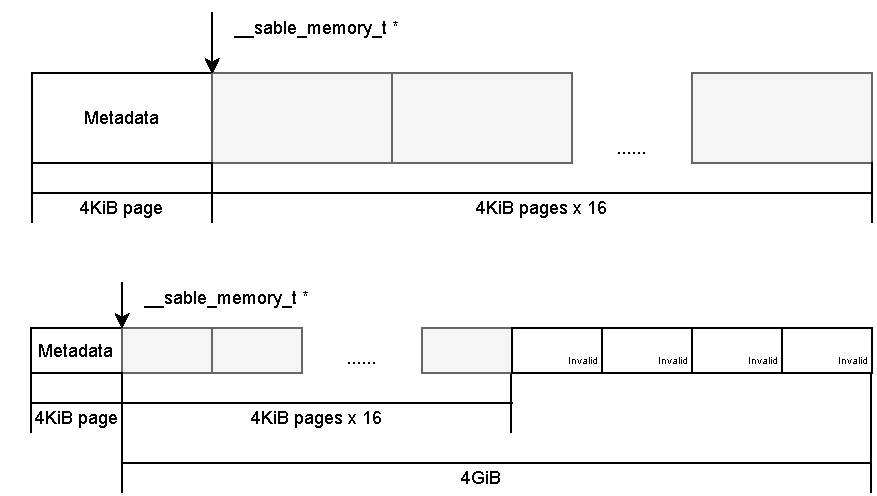
\includegraphics[width=0.85\textwidth]{Images/5.Backend and Runtime/memory}
    \caption{SableWasm WebAssembly linear memory}
    \label{fig:backend-memory}
\end{figure}

SableWasm implements WebAssembly linear memories with mapped memory provided
by the operating system. It also has a fallback implementation that uses
standard \texttt{malloc} and \texttt{free} procedure from the C library for an
operating system that does not support mapped memory. The fallback
implementation is relatively trivial, and we will not discuss it in the thesis.
Here, we will focus on the one that uses mapped memory.
Figure~\ref{fig:backend-memory} illustrates the strategies when mapping
WebAssembly linear memory into native memory. On the top, we have a linear
memory with a size of 1 in WebAssembly page size units, or 64KiB. In the figure,
we assume the native machine has a page size of 4KiB, which is typical for most
hardware architectures. Here's a quick recap on the requirements of WebAssembly
linear memories. First, the program can efficiently random access any location
within the linear memory. Second, at runtime, the module can query
the size of the linear memory. Finally, the program can grow the linear memory
if the runtime system allows it. SableWasm implements linear memories using
a similar trick as the one used for `\texttt{malloc}' functions in many C
standard library implementations. From the generated shared libraries'
perspective, the linear memory object points to the start of a continuous
memory chunk. Hence, memory accesses are efficient and require only one layer
of indirection. First, the generated function will fetch the linear memory base
pointer from the instance object and calculate offsets accordingly.
SableWasm also attaches an extra page that manages the metadata of the linear
memory at the beginning. It contains all the records that the runtime system
needs to work with the linear memory, such as the current size and the upper
bound. Note that the size of the metadata is usually way smaller than the page
size defined by the native machine. Still, SableWasm reserves a whole page for
it, as we want our linear memory start address to be always page-aligned in the
hope of better performance.

\begin{table}[h]
    \centering
    \begin{tabular}{|l|l|}
    \hline
    \textbf{Runtime builtin functions} & \textbf{Description}                              \\ \hline
    \_\_sable\_memory\_size            & Query for the size of the linear memory           \\ \hline
    \_\_sable\_memory\_guard           & Perform boundary check on the linear memory       \\ \hline
    \_\_sable\_memory\_grow            & Attempt to increase the size of the linear memory \\ \hline
\end{tabular}
    \caption{SableWasm runtime builtin functions for linear memory}
    \label{tbl:sablewasm-runtime-memory-api}
\end{table}

SableWasm implements additional functionalities through library functions.
Table~\ref{tbl:sablewasm-runtime-memory-api} illustrates all runtime library
builtin functions provided by SableWasm. \texttt{\_\_sable\_memory\_size}
implements SableWasm's \texttt{MemorySize} instruction. It takes an argument of
a linear memory instance and returns the size of it in WebAssembly page units.
The second runtime builtin function, \texttt{\_\_sable\_memory\_guard}
corresponds to the \texttt{MemoryGuard} instructions in SableWasm. It takes
a linear memory instance and the expected number of bytes ahead as arguments.
Note that the function does not return any values, and this is intentional
by design. SableWasm runtime library utilizes the C++ exception mechanism to
report and handle errors. If the memory access is out-of-bound, the runtime
system will throw an exception. We will come back to this later in this chapter
when discussing the interaction between generated shared libraries and the
host language. Finally, the last runtime builtin function,
\texttt{\_\_sable\_memory\_grow} implements the SableWasm's \texttt{MemoryGrow}
instruction. The instruction follows its counterpart that appeared in the
WebAssembly specification. It takes a linear memory instance and the number of
pages to increase as arguments. If the operation is successful, the function
will yield the new size of the linear memory; otherwise, it returns -1 instead.
SableWasm grows the memory by remapping the memory with the help of the
operating system. On Linux, this usually corresponds to a
\texttt{mremap} operation.

In the above implementation, all linear memory bounds checks are explicit and
program-directed, and thus they are relatively quite expensive. To further
improve the performance, we use a similar technique to that used by many
virtual machine implementations, which utilizes mapped memory access permission
flags. Figure~\ref{fig:backend-memory} illustrates this approach at the bottom.
One may notice that MVP WebAssembly works with 32-bit addressing
\footnote{This is subject to change in the future.
    WebAssembly 64-bit memory addressing:\\
    \url{https://github.com/WebAssembly/memory64}}. Hence, the maximum size of
the linear memory is 4GiB. Thus, SableWasm reserves 4GiB of address when
allocating a linear memory and marks all the pages beyond the current range as
invalid pages. This operation is quite efficient as it only works with the
memory address instead of allocating the memory. In this implementation, any
out-of-bound access will result in a memory segmentation fault. Note that this
strategy does yield better performance but results in a non-recoverable error.
SableWasm provides both implementations, and one can select based on their
needs. In the next chapter, when we compare SableWasm's performance against
several other implementations, we always use the second strategy, as the
recoverable code is not required.

\paragraph{Global}

\begin{figure}
    \centering
    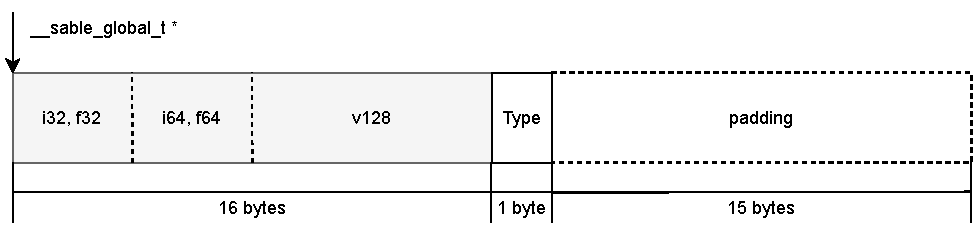
\includegraphics[width=\textwidth]{Images/5.Backend and Runtime/global}
    \caption{SableWasm WebAssembly linear global}
    \label{fig:backend-global}
\end{figure}

Compared to the WebAssembly linear memory implementation, SableWasm's
WebAssembly global variable implementation is relatively straightforward. In
the current version of WebAssembly, global variables can only store primitive
values. Therefore, SableWasm holds the WebAssembly global variable instance as
a union construct of all possible value types, followed by its type's character
encoding. Figure~\ref{fig:backend-global} illustrates SableWasm's implementation
for WebAssembly global variable instances. From the generated shared libraries'
perspective, the global variable access is equivalent to a simple load or store
operation. Note that, in generated shared libraries, we never need to worry
about the mutability of the global variables because the WebAssembly validation
rules ensure that a valid module should never write to a constant global
variable.

\paragraph{Indirect Table}
The last WebAssembly entity implemented in SableWasm is the indirect table, and
it perhaps is the most complex one among all three of them. A quick reminder,
in the instance layout section, we mentioned that we represent the function
instance in SableWasm using function closures that capture its enclosing
context. SableWasm implements the indirect table using a vector of function
closures and their type signatures. The internals of the SableWasm indirect
table is hidden from the generated shared libraries and only communicates to
them via runtime buitlin functions. Table~\ref{tbl:sablewasm-runtime-table-api}
illustrates all the runtime builtin functions provided by SableWasm for
indirect tables.

\begin{table}[h]
    \begin{tabular}{|l|l|}
    \hline
    \textbf{Runtime builtin functions} & \textbf{Description}                                        \\ \hline
    \_\_sable\_table\_guard            & Check if a given index is within the indirect table's range \\ \hline
    \_\_sable\_table\_check            & Check if the entry has specific type                        \\ \hline
    \_\_sable\_table\_context          & Fetch the context pointer of the entry                      \\ \hline
    \_\_sable\_table\_function         & Fetch the function pointer of the entry                     \\ \hline
    \_\_sable\_table\_set              & Write to indirect table                                     \\ \hline
\end{tabular}
    \caption{SableWasm runtime builtin functions for indirect table}
    \label{tbl:sablewasm-runtime-table-api}
\end{table}

\texttt{\_\_sable\_table\_guard} takes the indirect table instance and the
index as arguments. It is quite similar to \texttt{MemoryGuard} instructions,
except that it works with an indirect table. In addition, it also utilizes the
same error handling strategy by throwing an exception in the case where the
index is out-of-bounds. The next runtime builtin function,
\texttt{\_\_sable\_table\_check} implements the runtime type checking for
indirect function calls. It takes a pointer to an indirect table instance,
an index, and a function signature string as the parameter. We use the same
strategy as we have seen in the instance layout section to encode the
expecting type of the function. As in the current SableWasm, the type system is
extremely trivial, there is no complex typing judgment involved, such as
subtyping. Hence, the runtime type checking for indirect function calls is just
a simple string comparison. In the case of type mismatch, the runtime type
checking function also throws an exception. \texttt{\_\_sable\_table\_context}
and \texttt{\_\_sable\_table\_function} are the getter functions provided by
SableWasm. Both of them take an indirect table instance and an index as the
argument. These two functions assume the access is within range, and the
indirect table entry has the expected function type. We will come back to this
later in the chapter when we discuss the patterns used when lowering SableWasm
MIR into LLVM intermediate representations. As their names suggest, the first
function returns the pointer to the context instance object, and the second
function returns the function code address. Finally, the last runtime builtin
function for indirect tables is \texttt{\_\_sable\_table\_set}. Although in MVP
WebAssembly, indirect tables are immutable, the program cannot alter them after
they initialized \footnote{This is subject to change in the future. WebAssembly
    reference types:\\\url{https://github.com/WebAssembly/reference-types}},
the module initialization function still needs the setter function to setup
WebAssembly element segments. The setter function takes an indirect table
instance, an index, a function code address, and its null-terminated type
signature string as the argument. Similar to the getter functions, the setter
function assumes the index is always within range.

The SableWasm runtime library still provides another runtime builtin function
that does not fit into the categories above. SableWasm MIR defines an
\texttt{Unreachable} instruction, which should never reached by any control
flow, and if so, it will signal a runtime panic. In many other languages,
\texttt{Unreachable} maps to a hardware trap instruction, such as \texttt{ud2}
instruction on x86 architecture. However, this behaviour is not acceptable in
SableWasm. \texttt{ud2} generates a non-recoverable hardware invalid instruction
exception, which will eventually lead to the entire system core dump; on
the other hand, SableWasm expects exceptions thrown from generated shared
libraries and should handle them accordingly. Hence, the SableWasm runtime
library provides the \texttt{\_\_sable\_unreachable} function for the SableWasm
MIR \texttt{Unreachable} instruction. We will come back to this with more
details in the following section when discussing the code generation strategy
used when lowering SableWasm MIR into LLVM intermediate representation.
\section{Code Generation}
\label{section:runtime-codegen}

This section describes the code generation strategy used in the SableWasm LLVM
backend. For most of the instructions, especially for SableWasm MIR numeric
operations, the translation rules are simple mappings between SableWasm MIR
instructions and their LLVM counterparts. In this section, we will skip the
discussion over these trivial mapping. Instead, one can consult the SableWasm
source code for more details. The rest of the section will focus on several
key aspects: local variable implementation, linear memory manipulation,
indirect function calls, and SIMD instruction operations. One problem that
arises when lowering SableWasm MIR into LLVM intermediate representation is
how to pick the instruction translation order. Any instruction in SableWasm MIR
can refer to values either generated by a previous instruction in the same basic
block or instructions within a dominating block, implying that when lowering
SableWasm MIR, we need to perform a pre-order tree traversal over the dominator
tree. However, $\phi$ nodes may exist merging candidate values from prior
dominating blocks or due to subsequent backward branching.
Hence, the translation visitor may not have translated the candidate value
before $\phi$ nodes. SableWasm backend takes a two-phase translation to address
this problem. In the first pass, the backend will translate all the instructions
and collect the resulting values into a map, and in the second pass, the backend
will come back to the $\phi$ nodes and fix up the candidate values accordingly.

\paragraph{Function declaration and local variables} \quad
\begin{lstlisting}[
  basicstyle=\linespread{1}\small\ttfamily, 
  language=LLVM, 
  mathescape=true]
function %foo: [i32] -> [f32] {
  {(arg) %local0: i32, %local1: f64} 
  ......
}
$\Longrightarrow$
define private float @foo(%__sable_instance_t* %0, i32 %1) {
entry:
  %2 = alloca i32, align 4
  store i32 %1, i32* %2, align 4
  %3 = alloca double, align 8
  store double 0.000000e+00, double* %3, align 8
  ......
}

{%local: i32} 
%t0 = local.get %local $\Longrightarrow$ %t0 = load i32, i32* %local, align 4
local.set %local %t0 $\Longrightarrow$ store i32 %t0, i32* %local, align 4
\end{lstlisting}

We will first start by examining the translation pattern for lowering SableWasm
MIR functions into LLVM functions and their local variables. The example above
presents a simple function named \texttt{foo}, which takes a single 32-bit
integer as the argument and returns a single-precision floating-pointer number.
\texttt{foo} has two local variables. The parameter implicitly introduces the
first one, \texttt{local0}, and the function explicitly defines the second one,
\texttt{local1}. At runtime, \texttt{local0} will hold the value of the
parameter upon entry, and \texttt{local1} will initialize to zero. Compared to
the SableWasm MIR function definition, the one in LLVM intermediate
representation (IR) has three major differences. First, the LLVM function
definition has the extra instance object pointer in the arguments, in the
example above, \texttt{\%0}. We covered this briefly in the instance layout
section. In short, for all the functions, the SableWasm backend code generator
will implicitly add the instance object pointer as the first argument. The
second difference is in the entry block. SableWasm MIR, similar to WebAssembly,
views the local variables as opaque memory slots. However, LLVM IR requires
users to manually allocate them in stack memory space via the \texttt{alloca}
instruction. The \texttt{alloca} instruction reserves enough memory on the
stack based on the given type and returns a pointer. In example above,
\texttt{\%2} and \texttt{\%3} are two reserved local variable memory region
that correspond to \texttt{local0} and \texttt{local1} accordingly. The last
difference is that SableWasm IR defines implicit initialization for all local
variables; on the other hand, LLVM \texttt{alloca} instruction leaves the
reserved memory with uninitialized values. Hence, to faithfully implement
WebAssembly and SableWasm MIR specification, we generate \texttt{store}
instructions to set the initial values for each local variables. As for
\texttt{LocalGet} and \texttt{LocalSet} instructions, the translation patterns
are quite straightforward. The SableWasm backend code generator maps
\texttt{LocalGet} instructions to \texttt{load} instructions and
\texttt{LocalSet} instructions to \texttt{store} instructions as demonstrated
in the example above.

\paragraph{Linear memory operation} \quad
\begin{lstlisting}[
  basicstyle=\linespread{1}\small\ttfamily, 
  language=LLVM, 
  mathescape=true]
$\text{\textbf{Fetching linear memory:}}$
%t0     = getelementptr 
            inbounds %__sable_instance_t, %__sable_instance_t* %0, 
            i32 0, i32 4
%memory = load %__sable_memory_t*, %__sable_memory_t** %t0, align 8

%t0 = memory.size %mem $\Longrightarrow$
%t0 = call i32 @__sable_memory_size(%__sable_memory_t* %mem)
%t0 = memory.grow %mem %delta $\Longrightarrow$
%t0 = call i32 @__sable_memory_grow(%__sable_memory_t* %mem, i32 %delta)
memory.guard %mem %offset $\Longrightarrow$
call void @__sable_memory_guard(%__sable_memory_t* %mem, i32 %offset)
\end{lstlisting}
In section~\ref{section:runtime-instance-layout} and
\ref{section:runtime-webassembly-entities}, we presented how the
instance object manages the linear
memory instance and several runtime functions that implement additional
functionalities. The SableWasm backend code generator takes advantage of the
design by mapping SableWasm linear memory manipulation instructions into builtin
function invocations. The example above demonstrates the mapping for
\texttt{MemorySize}, \texttt{MemoryGrow} and \texttt{MemoryGuard} instructions.
All these instructions map to \texttt{call} instructions to their corresponding
builtin functions with appropriate arguments. Note that all builtin functions
require passing the linear memory pointer as an argument. Currently, the
WebAssembly module can have at most one linear memory. Due to the validation
rules, such linear memory must present within the module if linear memory
manipulation instructions appear in the program. Further, as we store linear
memory instance pointers before any other entities, one can show that the
linear pointer must be the 5th pointer in the instance object. Hence, the
SableWasm backend code generator fetches the linear memory instance pointer
using a pair of a \texttt{getelementptr} instruction and a \texttt{load}
instruction. The \texttt{getelementptr} instruction LLVM calculate addresses
for entries in a aggregation. The above example calculates addresses base on
the type \texttt{\_\_sable\_instance\_t} which is generated according to
declared entities at compile time.

\paragraph{Linear memory load and store} \quad
\begin{lstlisting}[
  basicstyle=\linespread{1}\small\ttfamily, 
  language=LLVM, 
  mathescape=true]
$\text{\textbf{Load a 32-bit integer:}}$
%result = load.32 i32 %mem %addr $\Longrightarrow$
  %t0     = ptrtoint %__sable_memory_t* %memory to i64
  %t1     = zext i32 %offset to i64
  %t2     = add nuw i64 %t0, %t1
  %addr   = inttoptr i64 %t2 to i32*
  %result = load i32, i32* %addr, align 1
$\text{\textbf{Partial load a 32-bit integer:}}$
%result = load.16 i32 %mem %addr $\Longrightarrow$
  ......
  %t0     = load i16, i16* %addr, align 1
  %result = zext i16 %t0 to i32
$\text{\textbf{Store a 32-bit integer:}}$
store.32 %mem %addr %val $\Longrightarrow$
  ......
  store i32 %val, i32* %addr, align 1
$\text{\textbf{Partial store a 32-bit integer:}}$
store.16 %mem %addr %val $\Longrightarrow$
  ...... 
  %t0    = trunc i32 %val to i16
  store i16 %t0, i16* %addr, align 1
\end{lstlisting}
SableWasm MIR classifies load and store instructions into two groups,
partial and complete. A quick reminder, WebAssembly associates load and store
operations with sign extension mode, while in SableWasm, we define load
instruction to perform zero extension, and store instructions always apply bit
truncation. The first example above presents a complete load operation for a
32-bit integer. The translation pattern is relatively straightforward. Note
that the linear memory instance pointer points to the first byte within the
linear memory. Hence, the SableWasm backend code generator will first calculate
the native write address by summing up offset and base pointer and map the
\texttt{Load} instruction to \texttt{load} in LLVM. The LLVM memory operation,
such as \texttt{load} and \texttt{store} has a complementary attribute,
\texttt{align}. In the background section, we introduced the attributes in
LLVM. In short, the \texttt{align} attribute marks an alignment requirement for
memory access operations. As WebAssembly linear memory is comparable to a byte
array, in which read-write can occur at any point, we can only conservatively
set the alignment to one in order to limit the LLVM backend instruction selector
from generating instructions with alignment assumptions. This, in theory, leads
to less efficient code. However, later in the evaluation section, we determine
this is not a bottleneck of the entire implementation. In the future, one can
further improve the performance of SableWasm by designing analyses that infer
lower bounds for alignment. The second example above demonstrates the
translation pattern for partial load operation. Compared to the complete load
instruction, the translation pattern for partial load instruction has an
additional zero-extending operation, \texttt{zext} at the bottom, to implement
the SableWasm MIR partial load semantics. On the other hand, the translation
pattern for both complete and partial \texttt{store} instructions are very
similar to \texttt{load} instructions. The most notable difference is the
\texttt{trunc} instruction in partial \texttt{store}'s translation pattern
which performs bit truncation on the operand.

\paragraph{Indirect function call} \quad
\begin{lstlisting}[
  basicstyle=\linespread{1}\small\ttfamily, 
  language=LLVM, 
  mathescape=true]
call.indirect %table %index %expect_ty $\Longrightarrow$ 
  call void @__sable_table_guard(%__sable_table_t* %table, i32 %index)
  call void @__sable_table_check(
    %__sable_table_t* %table, i32 %index, i8* %expect_ty)
  %t0 = call %__sable_instance_t* @__sable_table_context(
    %__sable_table_t* %table, i32 %index)
  %t1 = call %__sable_function_t* @__sable_table_function(
    %__sable_table_t* %table, i32 %index)
  %t2 = icmp eq %__sable_instance_t* %t0, null
  %t3 = select i1 %t2, %__sable_instance_t* %0, %__sable_instance_t* %t0
  %t4 = bitcast %__sable_function_t* %276 to ......
  %t5 = call ...... %t4(%__sable_instance_t* %t3, ......)
\end{lstlisting}
The SableWasm backend code generator implements indirect function calls via a
series of builtin function invocations. We have already presented the builtin
function in section~\ref{section:runtime-webassembly-entities}; hence, we will
not show them in detail in this
paragraph. The first step for calling an indirect function is to check if the
index is within range by calling the \texttt{\_\_sable\_table\_guard} builtin
function. If the index is within range, we then compare the expected function
type with the actual indirect function type with
\texttt{\_\_sable\_table\_check}. Note that this builtin function also checks
if the entry is a null function. If so, it will report an exception. The
SableWasm backend code generator uses a similar technique to encode the
expected function type into a null-terminated string, as we have seen in
section~\ref{section:runtime-instance-layout}. After we make sure the indirect
function is valid, we can now
fetch the context pointer and function address pointer by using two getter
functions, \texttt{\_\_sable\_table\_context} and
\texttt{\_\_sable\_table\_function}. Before we invoke the function, we need to
check if it is a host function. A quick reminder, SableWasm will set context
pointers for all host functions as null pointers, and when invoking a host
function, we need to pass the current instance object pointer as the context
pointer. The SableWasm code generator chooses the correct context pointer by
using a pair of \texttt{icmp} and \texttt{select} instruction. After selecting
the correct context pointer, the indirect function is straightforward by
casting the function code address into the function pointer and invoking it
appropriately. One may notice that the indirect function call in SableWasm is
costly and involves multiple function calls. WebAssembly specification does not
impose requirements on indirect function call efficiency, and later in our
benchmark, we determine that indirect function calls are not a performance
bottleneck. Hence, the SableWasm code generator focus on extensibility rather
than performance.

\paragraph{SIMD operation}
The last translation pattern we will cover in the section is the SIMD
operations. For most of the SIMD operations, the SableWasm backend code
generator maps to their LLVM counterparts. However, one challenge arises when
translating SableWasm MIR into LLVM intermediate representation around the
type system. In section~\ref{section:mir-opt-type-inference}, we presented the
type system for SableWasm MIR.
A quick reminder, the SableWasm MIR follows WebAssembly's design by erasing the
shape information from the vector values, depending on instructions to
interpret them correctly. However, LLVM intermediate representation does
require shape information for vectors. Hence, when lowering SableWasm MIR into
the LLVM intermediate representation, the SableWasm backend code generator needs
to insert cast instructions when required. For most of the numerical
instructions, this is pretty trivial. The backend code generator will first
infer an LLVM vector type based on the SableWasm instruction shape information.
For example, \texttt{v128.add i16x4} implies that the operand must have type
\texttt{<4 x i16>} in LLVM. In the case where the shape type is unsuitable,
the SableWasm backend code generator will insert a bit cast,
\texttt{bitcast to}. The bit cast operation is always valid as, in the current
version of SableWasm MIR, we only work with 128-bit vectors. However, there
are still several corner cases in this strategy. What type should we assign to
$\phi$ nodes when merging vectors from multiple control-flow? Also, what type
should we assign for load instruction when shape information is still not yet
available? The SableWasm backend code generator takes advantage of the fact
that integer types in LLVM can be arbitrarily long, and more specifically,
128-bit integer, \texttt{i128}, is a valid type in LLVM. The SableWasm backend
code generator will always use \texttt{i128} as a default type in these corner
cases. For example, for load instruction for SableWasm vectors, the code
generator will emit a \texttt{load} instruction with \texttt{i128} type, and
later when any instruction takes the value as the operand, it will setup the
bit cast instruction accordingly.
\section{Interface with C/C++}
The last section of this chapter will cover the interface between the generated
shared library and the host languages. Currently, SableWasm only has a binder
library for C/C++. However, the principle is relatively straightforward, and
one can add implementations of the binder function for any other language. In
the rest of the section, we will focus our discussion on the callee wrapper,
WASI function implementations and error handling strategies.

\paragraph{Callee wrapper}
Section 5.2 mentioned that SableWasm stores a function instance as a pair of
context pointer and function address pointer. Additionally, SableWasm also
encodes the function types as null-terminated strings. However, all this
information is only available to the host program at runtime. C/C++ is a
statically typed language; hence, we can only specify type contracts on the
exported functions at compile-time and verify the contracts at runtime.
Traditionally, one can use a type erased pointer, a \texttt{void} pointer,
to store the function address and reinterpret it to the actual concrete type.
SableWasm presents a helper class that provides type-safe access to the
exported functions: \texttt{WebAssemblyCallee}. \texttt{WebAssemblyCallee} takes
advantage of the template metaprogramming system in C++ and generates
a null-terminated encoding of an expected type at compile-time. At runtime,
the wrapper class will check the type signature string against the actual type
string before forwarding the function call. If the type signature string does
not match, the system will signal an exception.

\paragraph{WASI interface implementation}
WebAssembly System Interface (WASI) extends WebAssembly by providing syscalls
that interact with the host environment. This extension is non-invasive, and
all the syscalls are in the form of imported functions, mainly host
functions. Hence, SableWasm implements the WASI extension using host library
functions only. At the shared library initialization phase, the loader will set
up WASI host functions based on the import descriptor. Currently, SableWasm only
implements the minimal WASI interface functions necessary in order to run
benchmarks, such as standard I/O and timing. However, the framework is easy to
extend, and all the WASI function implementations are under the namespace
\texttt{runtime::wasi}. Therefore, we will skip them in detail in the thesis;
one can consult the source code for implementation details of WASI interface
functions. One of the project's future work is to continuously work on the
WASI system interface and add more features to SableWasm, such as
capability-based file system and networking.

\paragraph{Error handling strategies}
The last topic we will address in the section is error handling. SableWasm
builds its error handling strategy based on the C++ exception mechanism.
Comparing to other exception handling strategies, this brings us two
significant benefits. First, when generating LLVM intermediate representation
for shared libraries, we can avoid boilerplate code that propagates exceptions.
Additionally, on most modern system ABIs that supports zero-cost exception
handling, this gives SableWasm a performance advantage. On the other hand, this
leaves us room for further improvement for pending WebAssembly extensions, such
as the WebAssembly exception handling extension \footnote{WebAssembly exception
    handling: \url{https://github.com/WebAssembly/exception-handling}}.
The WebAssembly exception handling extension generalizes the WebAssembly
specification by adding \texttt{try catch} construct to the syntax, which
directly corresponds to the C++ exception handling mechanism.

\begin{figure}
    \centering
    \lstinputlisting[
        language=C++,
        basicstyle=\linespread{0.8}\small\ttfamily,
        numbers=left
    ]{Code/Tester.cc}
    \caption{Simple C++ SableWasm loader function}
    \label{fig:sablewasm-loader}
\end{figure}

In this section, we discussed the interaction between C/C++ and the SableWasm
system. We will conclude the chapter with a concrete loader function example.
Figure~\ref{fig:sablewasm-loader} demonstrates a simple loader function for
generated SableWasm shared libraries. In the example above, we assume the
WebAssembly module is a WASI compatible module, and hence, exports a function
named \texttt{\_start} as the entry function with type \texttt{[] -> []}.

